 \documentclass[17pt]{article}
\usepackage{fancyhdr} % Required for custom headers
\usepackage{lastpage} % Required to determine the last page for the footer
\usepackage{extramarks} % Required for headers and footers
\usepackage{graphicx} % Required to insert images
\usepackage{lipsum} % Used for inserting dummy 'Lorem ipsum' text into the template
\usepackage{amsmath,amsthm,amsxtra}

% Margins
\topmargin=-0.45in
\evensidemargin=0in
\oddsidemargin=0in
\textwidth=6.5in
\textheight=9.0in
\headsep=0.25in 

\linespread{1.1} % Line spacing

% Set up the header and footer
\pagestyle{fancy}
\lhead{\hmwkAuthorName} % Top left header
\chead{\courseTitle\ : \hmwkTitle} % Top center header
\rhead{\firstxmark} % Top right header
\lfoot{\lastxmark} % Bottom left footer
\cfoot{} % Bottom center footer
\rfoot{Page\ \thepage\ of\ \pageref{LastPage}} % Bottom right footer
\renewcommand\headrulewidth{0.4pt} % Size of the header rule
\renewcommand\footrulewidth{0.4pt} % Size of the footer rule

\setlength\parindent{0pt} % Removes all indentation from paragraphs

%----------------------------------------------------------------------------------------
%	DOCUMENT STRUCTURE COMMANDS
%	Skip this unless you know what you're doing
%----------------------------------------------------------------------------------------

% Header and footer for when a page split occurs within a problem environment
\newcommand{\enterProblemHeader}[1]{
\nobreak\extramarks{#1}{#1 continued on next page\ldots}\nobreak
\nobreak\extramarks{#1 (continued)}{#1 continued on next page\ldots}\nobreak
}

% Header and footer for when a page split occurs between problem environments
\newcommand{\exitProblemHeader}[1]{
\nobreak\extramarks{#1 (continued)}{#1 continued on next page\ldots}\nobreak
\nobreak\extramarks{#1}{}\nobreak
}

\setcounter{secnumdepth}{0} % Removes default section numbers
\newcounter{homeworkProblemCounter} % Creates a counter to keep track of the number of problems
\newcommand{\homeworkProblemName}{}
\newenvironment{homeworkProblem}[1][Problem \arabic{homeworkProblemCounter}]{ % Makes a new environment called homeworkProblem which takes 1 argument (custom name) but the default is "Problem #"
\stepcounter{homeworkProblemCounter} % Increase counter for number of problems
\renewcommand{\homeworkProblemName}{#1} % Assign \homeworkProblemName the name of the problem
\section{\homeworkProblemName} % Make a section in the document with the custom problem count
\enterProblemHeader{\homeworkProblemName} % Header and footer within the environment
}{
\exitProblemHeader{\homeworkProblemName} % Header and footer after the environment
}

\newcommand{\problemAnswer}[1]{ % Defines the problem answer command with the content as the only argument
\noindent\framebox[\columnwidth][c]{\begin{minipage}{0.98\columnwidth}#1\end{minipage}} % Makes the box around the problem answer and puts the content inside
}

\newcommand{\homeworkSectionName}{}
\newenvironment{homeworkSection}[1]{ % New environment for sections within homework problems, takes 1 argument - the name of the section
\renewcommand{\homeworkSectionName}{#1} % Assign \homeworkSectionName to the name of the section from the environment argument
\subsection{\homeworkSectionName} % Make a subsection with the custom name of the subsection
\enterProblemHeader{\homeworkProblemName} % Header and footer within the environment
}{
\enterProblemHeader{\homeworkProblemName} % Header and footer after the environment
}

%----------------------------------------------------------------------------------------
%	NAME AND CLASS SECTION
%----------------------------------------------------------------------------------------

\newcommand{\hmwkTitle}{Assignment 1} % Assignment title
\newcommand{\hmwkDueDate}{Wendesday,\ January\ 30,\ 2013} % Due date
\newcommand{\courseTitle}{Physics 760: Electricity and Magnetism} % Course/class
\newcommand{\hmwkClassInstructor}{Dr. Stefan Kycia} % Teacher/lecturer
\newcommand{\hmwkAuthorName}{John Rinehart} % Your name
\newcommand{\sudentNumber}{20503440} % Your name
\newcommand{\position}{PhD student at ECE departent}

%----------------------------------------------------------------------------------------
%%-----------------------------------------------------------------------------------------

%%%%%%%%%%
\newcommand{\red}[1]{\textcolor[rgb]{1,0,0}{#1}}
\newcommand{\blu}[1]{\textcolor[rgb]{0,0,1}{#1}}
\newcommand{\bs}[1]{\boldsymbol{#1}}
%\newcommand{\V}[1]{\bm{#1}}
\newcommand{\V}[1]{\Vec{#1}}
\newcommand{\A}[1]{\Hat{#1}}
\newcommand{\W}[1]{\widehat{#1}}
\newcommand{\T}[1]{\widetilde{#1}}
\newcommand{\pd}[2]{\dfrac{\partial #1}{\partial #2}}
\newcommand{\fpd}[2]{\frac{\partial #1}{\partial #2}}
\newcommand{\pds}[1]{\dfrac{\partial}{\partial #1}}
\newcommand{\fpds}[1]{\frac{\partial}{\partial #1}}
\newcommand{\pdss}[1]{\dfrac{\partial^2}{\partial {#1}^2}}
\newcommand{\pdsss}[2]{\dfrac{\partial^2}{\partial #1 \partial #2}}
\newcommand{\pdt}[2]{\dfrac{\partial^2 {#1}}{\partial {#2}^2}}
\newcommand{\pdtt}[3]{\dfrac{\partial^2 {#1}}{\partial {#2} \partial {#3}}}
\newcommand{\dif}[2]{\frac{d{#1}}{d{#2}}}
\newcommand{\vt}[1]{\Vec{\mathcal{#1}}}
\newcommand{\VP}[1]{\Vec{\mathbf{#1}}}
\newcommand{\vp}[1]{\mathbf{#1}}
\newcommand{\phas}[1]{\angle{#1}^{\circ}}
\newcommand{\er}{\epsilon_{r}}
\newcommand{\mr}{\mu_{r}}
\newcommand{\Lrw}{\Longrightarrow}
\newcommand{\refeq}[1]{(\ref{#1})}
\newcommand{\abs}[1]{\left| #1\right|}
\newcommand{\ket}[1]{|#1\rangle}
\newcommand{\bra}[1]{\langle #1| }
\newcommand{\bracket}[2]{\langle#1|#2\rangle }


%%%---
\newcommand\ointint{\begingroup
\displaystyle \unitlength 1pt
\int\mkern-7.2mu
\begin{picture}(0,3)
\put(0,3){\oval(10,8)}
\end{picture}
\mkern-7mu\int\endgroup}
%%%----
\providecommand{\abs}[1]{\lvert#1\rvert}
\providecommand{\norm}[1]{\lVert#1\rVert}

%%%%%%%%%%%%%%%

%---Packeges------------------------------------------------------------------
 %------------------------------------------------------
\usepackage[utf8]{inputenc}
\usepackage[T1]{fontenc}
\usepackage[english]{babel}
\usepackage[latin1]{inputenc}
\usepackage[T1]{fontenc}
\usepackage{pstricks}
\usepackage[usenames,dvipsnames]{pstricks}
\usepackage{epsfig}
\usepackage{pst-grad} % For gradients \usepackage{pst-plot} % For axes
\usepackage{pifont}
\usepackage{amsfonts}
\graphicspath{{IMG/}}
\usepackage[utf8]{inputenc}
 \usepackage[OT1]{fontenc}
 \usepackage[absolute,overlay]{textpos}
 \usepackage{graphicx}
 \usepackage[bookmarks=false,pdffitwindow]{hyperref}
 \usepackage{tikz}
 \usepackage{xcolor}
 \usepackage{calc}
\usepackage{chngcntr}
%----------------------------------------------------------------
\numberwithin{equation}{section}
\renewcommand{\theequation}{\arabic{equation}}



%%------------------------------------------------------------------------------------------
%	TITLE PAGE
%----------------------------------------------------------------------------------------

\title{
\vspace{2in}
\textmd{\textbf{\courseTitle\\ \vspace{0.5in}\hmwkTitle}}\\
\vspace{0.5in}\large{{\hmwkClassInstructor}}
\vspace{3in}
}
\author{\textbf{\hmwkAuthorName}\\ 
}\\
\date{January 1, 2000} % Insert date here if you want it to appear below your name

%----------------------------------------------------------------------------------------

\begin{document}

\maketitle


\newpage
\tableofcontents
\newpage


%----Problems-------
\begin{homeworkProblem}
\textbf{A plane wave is incident normally from air ($n_1 =1$) on a plane slab of a transparent dielectric material with index of refraction $n_2$ and of thickness $d$. The light passes the slab and enters a third
medium with index of refraction $n_3$ and of infinite extent.}
\begin{homeworkSection}{a}
\textbf{Calculate the reflection coefficient R as a function of the thickness $d$ for monochromatic light of
wavelength $\lambda_0$ . Plot R as a function of $d$ for $n_3 =1.5$ and $n_2 =1.0, 1.2$ and  $3.0$.}
\\

As the wave travels through the medium with index of refraction $n_2$ it will acquire phase 
relative to the incident wave. Consider a wave that is incident on the slab of material 2 
at some angle $\theta_1$ relative to the normal to the surface. Some of the wave will be transmitted into material 2. This portion will have some fraction of itself reflect off the surface where 
material 3 meets material 2. If we compare the phase of the wave at the point that it 
first entered material 2 with the phase that it has when it reaches a point in its path that 
intersects the perpendicular to the initial direction of the wave when it entered material 
2 we will really be finding the phase difference between adjacent plane waves that are 
formed by reflections off material 3.
\\

To find this ``distance to the perpendicular'', consider the wave after the reflection off of 
material 3. It will first travel through 
a distance of $l_1 = \frac{d}{\cos\theta_2}$. The wave will travel another distance to reach the point where it intersects the perpendicular of the wavefront which can be shown to be 
$l_2 = \frac{d}{\cos\theta_2}\sin(\pi-(\pi/2+2\theta_2))$. Summing $l_1$ with $l_2$ and using 
some trigonometric identities, the total distance $l$ traveled through material before the 
wave reaches the ``next plane'' can be shown to be $\delta_l = 2d\cos\theta_2$. The phase 
difference between the two fictitious plane waves (the original plane wave and a time-advanced 
version of that wave is given by the $\vec{k}\cdot\vec{x}$ in the exponential describing the 
plane wave. Thus, the phase difference is $\delta_{\phi} = \frac{2\pi}{\lambda_2}\delta_l = 
\frac{4\pi}{\lambda_2}d \cos\theta_2$. In the case of normal incidence this expression 
reduces to $\delta_{\phi} = \frac{4\pi d}{\lambda_2}$.
\\

The above was necessary in order to perform the folowing steps. See, depending on the indices 
of refraction $n_1, n_2, \,\text{and}\, n_3$ the wave will reflect an infinite number of times 
between the two surfaces (where material 1 meets material 2 and, also, where material 2 
meets material 3. Each time it encounters an interface some portion of the wave will get 
reflected and some portion will be transmitted. Because of the thickness of material 2, the 
wave will also acquire a complex phase which will result in one reflected and/or transmitted 
wave's interference with all of the other instances of reflection or transmission.
\\

Consider a ray of light incident normally to the surface where materal 1 meets material 2. Assign this light a plane wave of the form $\vec{E_I}(\vec{x},t) = \vec{E_0}\exp(i(\vec{k}\cdot\vec{x}-\omega t))$. The first transmitted wave will have the form $\vec{E_{t_1}} = \vec{E_0}*t_{21}*\exp(i(\vec{k_2}\cdot\vec{x}-\omega t))*\exp(i\phi)$. $\phi$ in the previous expression accounts for the accumulation of the wave's phase as it travels though material 2 towards material 3. Note, also, that I have introduced a notation that I will use throughout the rest of this problem set. $t_{ij}$ is the scaling factor for waves which are transmitted from region j into region i. Similarly, $r_{ij}$ is the scaling factor for waves which are reflected off material j into material i. Explicit expressions for these are:

\begin{align*}
  t_{ij} &= 2\frac{n_j}{n_i+n_j} \\ 
  r_{ij} &= \frac{n_i-n_j}{n_i+n_j}
\end{align*}
\\

It is sufficient to consider just the amplitude of the wave from this point on. That is, I can safely drop the time component since I am dealing with monochromatic light and the time dependence is the same between all generated rays. The sum of all of the complex amplitudes of the transmitted rays will give me the amplitude of the resultant wave.
\\

Now, I will define a reference for the phase in this problem. The reference phase is that of the first wave immediately after it has exited the 3rd material (or, equivalently, as soon as it encounters the interface). Subsequent transmissions (due to reflections off of the interface between material 2 and material 3) will acquire a phase determined by the total distance traveled through the material. Thus, utilizing this definition and the fact that I can disregard the time component of the wave, I can express the ray that is first transmitted into material 3 as : $\vec{E}_{t_1} = \vec{E_0}*t_{21}*t_{32}$.
\\

Now, part of the incident wave makes it in the ``first pass'' to material 3. Some of this wave is reflected before any of the wave is transmitted into material 2. Some of the wave is transmitted into material 2 (this is the wave we have just considered). However, after this wave encounters material 3 a portion of this wave may be reflected at this interface. Thus, a new wave will later exit material 2 into material 3 and we must consider this wave's interference with our first wave.
\\

Utilizing the prior disussion regarding the acquired phase. I may write that the complex amplitude of the wave due to the transmission into material 1, reflections off of the two interfaces, transmission into material 3 and total distance traveled through material 2 as : $\vec{E}_{t_2} = \vec{E_0}*t_{21}*r_{23}*r_{21}*t_{32}*exp(i\frac{4\pi d}{\lambda_2}) = \vec{E}_{t_1}*r_{23}*r_{21}*exp(i\phi)$. I will omit the vector arrow above $E_0$ for brevity. I still maintain that it is a complex vector quantity. I will also allow the phase acquired due to the thickness of the plate to be designated as $\phi$. 
\\

Although we have discovered the amplitude of the second ray to penetrate material 3 we must consider that some of this ray reflected at the interface between material 2 and 3 and thus, there is a 3rd ray that will exit material 2 into material 3. Its amplitude is described by: $E_0*t_{21}*r_{23}*r_{21}*r_{23}*r_{21}*t_{23}*\exp(2 i\phi) = E_{t_2}*r_{23}*r_{21}*exp(i\phi) = E_{t_1}* (r_{23}*r_{21}*exp(i\phi))^2$.
\\

It is clear that this trend will continue ad infinitum and that the amplitude of the nth transmitted wave can be described as $E_{t_n} = E_0*t_{21}*t_{32}*(r_{23}*r_{21}*exp(i*\phi))^n$. Thus, the net wave will have an amplitude $E_t = \sum\limits_{n=0}^\infty E_0 t_{21} t_{32} (r_{23}r_{21}\exp(i\phi))^n$. This is a simple geometric series with solution $E_t = E_0 t_{21} t_{32} \frac{1}{1-r_{23}r_{21}\exp(i\phi)}$. To find the transmission coefficient T I will first normalize the transmitted wave amplitude by the incident wave. Then, I will multiply the wave amplitude by its complex conjugate. This is not complete, though. The transmission coeffecient is defined as the ratio of the transmited power per unit area and the incident power per unit area. The power per unit area is given by $\frac{1}{2}\sqrt{\epsilon}{\mu}|E_0|^2$. This can be expressed in terms of $n$ (the index of refraction of the material) as $\frac{1}{2} \sqrt{n}{c\mu}|E_0^2$. Thus, the intensity of light in the third medium divided by the intensity of light in the first medium would be given by $T = \frac{n_3}{n_1} \frac{|E_t|^2}{|E_I^2|}$.
\\

Using the previous expression and explicitly avoiding typing a lot of tedious algebra: 

\begin{problemAnswer}{
T = \frac{n_3}{n_1}|\frac{E_t}{E_0}|^2 =\frac{n_3}{n_1} \frac{(t_{21}t_{32})^2}{1-(r_{23}r_{21})^2-2 r_{23} r_{21} \cos\phi }}
\end{problemAnswer}

$\phi$ in terms of the wavelength in vacuum is $\phi = \frac{4\pi n_2}{\lambda_0}d$. I have plotted this transmission coefficient in Figure 1 as $n_2$ takes on different values. $n_1$ and $n_3$ are 1 and 1.5, respectively.

\begin{figure}
  \centering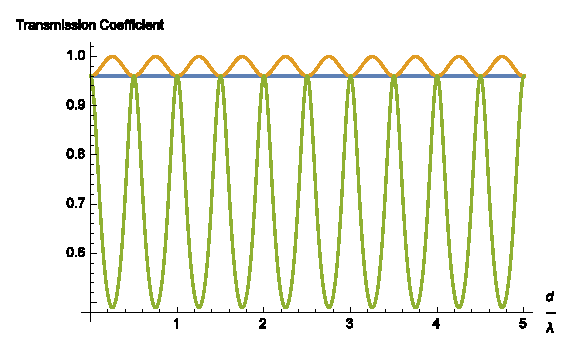
\includegraphics[width=.5\textwidth]{Images/TransCoef.eps}
  \caption{Transmission coefficient with $n_2$ = 1.5 (green), 1 (blue), 1.2 (orange) }
\end{figure}
\end{homeworkSection}

\begin{homeworkSection}{b}
\textbf{Calculate the Transmission coefficient T (transmission of incident wave into the third medium)
as a function of the thickness d for monochromatic light of wavelength $\lambda_0$ . Plot T as a function of
d for $n_3 =1.5$ and $n_2 =1.0, 1.2$ and $3.0$.}
\\

The analysis for this part of the problem will be very similar to the previous problem. The zeroth wave that is reflected will have amplitude $E_{r_0} = E_0*r_{12}$. The first wave will be related to the incident wave by $E_{r_1} = E_0*t_{21}*r_{23}*t_{12}*\exp(i\phi)$. Here, $\phi$ has the same form it did before. The second wave will have amplitude: $E_{r_2} = E_0*t_{21}*r_{23}*r_{21}*r_{23}*t_{12}*\exp(2 i\phi) = E_{r_1} * r_{21}*r_{23}*\exp(i\phi)$. The third wave will bear the same relationship with the second wave as the second wave has with the first $E_{r_3} = E_{r_2} *r_{21} * r_{23}*\exp(i\phi) = E_{r_1} * (r_{21}*r_{23})^2*\exp(2i\phi)$. Thus, it seems that the $E_{n>0}$ wave can be expressed as $E_{n} = E_{r_1}(r_{21}*r_{23}*exp(i\phi))^{n-1}$.
\\
Thus, the reflected amplitude is $E_{r} = E_{r_0} + \sum\limits_{n=1}^\infty E_{r_1}(r_{21}*r_{23}*\exp(i\phi))^{n-1}$. Recognizing the geometric series, again, and simplifying the resulting expression yields: $E_0 r_{12} + \frac{E_0 t_{21}r_{23}t_{12}\exp(i\phi)}{1-r_{23}r_{21}\exp(i\phi)}$. Taking the magnitude squared of this expression yields the reflection coefficient $R = |\frac{E_r}{E_0}|^2 = (\frac{\alpha^2 + 2 \alpha r_{12}\cos\delta\phi - 2\alpha r_{12}r_{21}r_{23}}{1+(r_{21}r_{23})^2-2 r_{21} r_{23} \cos\delta\phi} + r_{12}^2)$. $\alpha = t_{21}t_{12}r_{23}$: Substituting this into my previous expression, factoring and simplifying yields:
\begin{problemAnswer}{
R = \frac{r_{12}^2+r_{23}^2+2r_{12} r_{23}\cos\delta\phi}{1+r_{23}^2r_{21}^2-2r_{23}r_{21}\cos\delta\phi}
}
\end{problemAnswer}

I have plotted this in the second figure for the same $n_1, n_2 \,\text{and}\, n_3$ values as before for the transmission coefficient. Note that the sum of each of the corresponding plots yields 1 at any choice of the thickness of the plates.

\begin{figure}
  \centering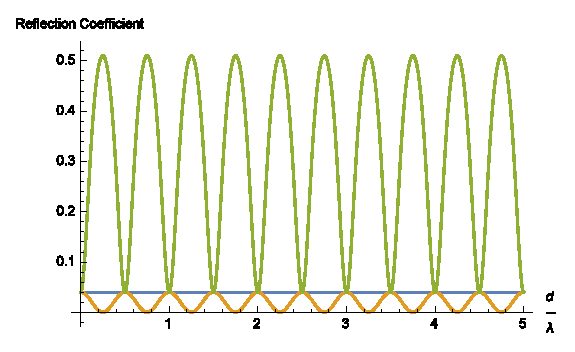
\includegraphics[width=.5\textwidth]{Images/RefCoef.eps}
  \caption{Transmission coefficient with $n_2$ = 1.5 (green), 1 (blue), 1.2 (orange)}
\end{figure}

\end{homeworkSection}

\begin{homeworkSection}{c}
An obvious application of this device is that of filtering a particular frequency of light. One could tune the distance of separation between material 1 and 3 to result in total interference in the transmission. Another application could be in using a variable distance (variable d) apparatus to experimentally determine the particular wavelength of light being generated by a monochromatic source.
\end{homeworkSection}
\end{homeworkProblem}

\setcounter{equation}{0}
%---------------------
% Problem 2
\begin{homeworkProblem}[Problem 2: Unilateral Power Spectral Density]
   \problemStatement{
In class, we examined one example with a noisy waveform $x(t)$, which is a
wide-sense statistically stationary. The autocorrelation function $
\phi_{x}(\tau) $ has a form of
\[
   \phi_{x}(\tau) = \phi_{x}(0)\exp(- \frac{|\tau|}{\tau_1})
\]
where $ \tau_1 $ is a relaxation time constant.  Compute the unilateral power
spectral density $ S_{x}(\omega) $ using the Wiener-Khintchine theorem.}

Using the Wiener-Khintchine theorem, we have:
\begin{align*}
   S_{x}(\omega) &= 4 \int_0^{\infty} \phi_{x}(0) \exp(-\frac{|\tau|}{\tau_1}) \cos(\omega
\tau) d \tau \\
&= 4 \phi_{x}(0) \int_{0}^{\infty} \exp(-\frac{|\tau|}{\tau_1}) \cos(\omega
\tau) d \tau
\intertext{Now, substituting $ \cos(\omega \tau) = .5 \left( \exp(i \omega \tau)
+ \exp(-i \omega \tau)\right) $.}
&= 2\phi_{x}(0) \int_{0}^{\infty} \exp(-\frac{|\tau|}{\tau_1}) \left( \exp(i \omega \tau)
+ \exp(-i \omega \tau)\right) d \tau \\
&= 2\phi_{x}(0) \int_{0}^{\infty} \exp(-\frac{|\tau|}{\tau_1}) \exp(i \omega \tau) d \tau +
2\phi_{x}(0) \int_{0}^{\infty} \exp(-\frac{|\tau|}{\tau_1}) \exp(-i \omega \tau)
d \tau \\
\intertext{Because the integral bounds are only over positive $ \tau $, the
absolute values signs are redundant. They will now be dropped.}
&= 2\phi_{x}(0) \int_{0}^{\infty} \exp(\frac{-\tau}{\tau_1}+i \omega \tau) d \tau +
2\phi_{x}(0) \int_{0}^{\infty} \exp(-\frac{\tau}{\tau_1}-i \omega \tau)
d \tau \\
&= 2\phi_{x}(0) \frac{\exp(\frac{-\tau}{\tau_1}+i \omega
\tau)}{\frac{-1}{\tau_1} + i\omega}\bigg|_{\tau=0}^{\infty} +
2\phi_{x}(0) \frac{\exp(\frac{-\tau}{\tau_1}-i \omega
\tau)}{\frac{-1}{\tau_1} - i\omega}\bigg|_{\tau=0}^{\infty} \\
\intertext{The upper bounds for both integrals clearly yields $ 0 $. All that
remains is the lower bound.}
&= 2\phi_{x}(0) \frac{\tau_{1}}{1-i \omega \tau_{1}} +
2\phi_{x}(0) \frac{\tau_{1}}{1 + i \omega \tau_{1}} \\
&= 2\phi_{x}(0) \frac{\tau_{1}\left( 1+ i \omega \tau_{1} \right) +
\tau_{1}\left( 1-i\omega\tau_{1}  \right)}{1+\omega^2 \tau_{1}^{2}} \\
&= 4\phi_{x}(0) \frac{\tau_{1}}{1+\omega^2 \tau_{1}^{2}}
\end{align*}
This is a Lorentzian-type function of $ \tau_1 $.
\end{homeworkProblem}

\setcounter{equation}{0}
%--------------------- 
%%%\begin{homeworkProblem}
The spinor part of the Hamiltonian describing time evolution of  an half spin system such as electron inside a uniform but time-varying magnetic filed is:
\begin{equation}
H=-\B{\mu}.\vp{B}=-\frac{gq}{2m}\vp{S}.\vp{B}=-\mu_0\B{\sigma}.\vp{B}
\end{equation}
 where $g$ is gyromagnetic ration and $\mu_0$ is defined as:
 \begin{equation}
 \mu_0=\frac{qg}{2m}
 \end{equation}
Explicitly the Hamiltonian is:
\begin{equation}
H=-\mu_0B_0
\begin{pmatrix}
\cos\theta & \sin\theta\left[\cos\omega t-i\sin\omega t\right]\\
\sin\theta\left[\cos\omega t+i\sin\omega t\right] & -\cos\theta
\end{pmatrix}
\end{equation} 
For notational convenience we write the Hamiltonian in terms of two new parameters:
\begin{equation}
H=-\hbar
\begin{pmatrix}
\omega_1              & \gamma e^{-i\omega t}\\
\gamma e^{i\omega t} & -\omega_1 
\end{pmatrix}
\end{equation}
where:
\begin{align*}
\hbar\omega_1 &=\mu_0B_0\cos\theta\\
 \hbar\gamma &=\mu_0B_0\sin\theta
\end{align*}
The Schr\"odinger equation now reads:
\begin{equation}\label{P3-S}
i\hbar\frac{d}{dt}
\begin{pmatrix}
c_1(t)\\
c_2(t)
\end{pmatrix}
=
-\hbar\begin{pmatrix}
\omega_1              & \gamma e^{-i\omega t}\\
\gamma e^{i\omega t} & -\omega_1 
\end{pmatrix}
\begin{pmatrix}
c_1(t)\\
c_2(t)
\end{pmatrix}
\end{equation}
In the absense of the time dependent part of the Hamiltonian the solution is simply $c_1(t)=A\exp(i\omega_1 t)$ and $c_2(t)=B\exp(-i\omega_1 t)$. It's reasonable to keep the exponential part for the new Hamiltonian. Two coupled first order differential equations given in \eqref{P3-S} can be extremely simplified by the following change of varibles:
\begin{equation}
c_1(t)=A(t)\exp(i\omega_1 t)\qquad  c_2(t)=B(t)\exp(-i\omega_1 t)
\end{equation}   
Two new coupled equations are:  
\begin{equation}
\left\{
\begin{array}{l}
i\frac{dA(t)}{dt}=-\gamma \exp\left[-i(\omega +2\omega_1)t\right]B(t)\\
i\frac{dB(t)}{dt}=-\gamma \exp\left[+i(\omega +2\omega_1)t\right] A(t)
\end{array}\right.
\end{equation}
If we solve $B(t)$ from the first equation and put it in the second one, we obtain:
\begin{equation}
\frac{d^2A}{dt^2}+i\alpha \frac{dA}{dt}+\gamma^2 A=0
\end{equation}
where $\alpha$ has been defined for notational convenience:
\begin{equation}
\alpha=\omega+2\omega_1
\end{equation}
because of symmetry the same equation holds for $B(t)$ we should change the sign of $\alpha$:
\begin{equation}
\frac{d^2B}{dt^2}-i\alpha \frac{dB}{dt}+\gamma^2 B=0
\end{equation}  
The general solution for two differential equations are simply:
\begin{align}
&A(t)=A_{+} \exp(i\Omega_+t)+A_-\exp(i\Omega_-t)\\
&B(t)=B_+\exp(-i\Omega_+t)+B_-\exp(-i\Omega_-t)
\end{align}
where $\Omega_+$ and $\Omega_-$ are defined as:
\begin{equation}
\Omega_\pm=-\frac{\alpha}{2}\pm\sqrt{\frac{\alpha^2}{4}+\gamma^2}
\end{equation}
The constant coefficients can be writen in terms of $A(0)$ and $B(0)$ :
\begin{equation}
\left\{
\begin{array}{rcl}
A(0) &=&A_++A_- &\\
B(0) &=&B_++B_- &\\
\left.\frac{dA}{dt}\right|_{t=0}=i\gamma B(0)&=&+i\Omega_+A_++i\Omega_-A_-\\
\left.\frac{dB}{dt}\right|_{t=0}=i\gamma A(0)&=&-i\Omega_+B_+-i\Omega_-B_-
\end{array}\right.
\end{equation}
These eqquation lead to:
\begin{align}
A_+&=\frac{\Omega_+ A(0)-\gamma B(0)}{\Omega_+-\Omega_-}\\
A_-&=-\frac{\Omega_+ A(0)-\gamma B(0)}{\Omega_+-\Omega_-}\\
B_+&=-\frac{\Omega_- B(0)+\gamma A(0)}{\Omega_+-\Omega_-}\\
B_-&=\frac{\Omega_+ B(0)+\gamma a(0)}{\Omega_+-\Omega_-}
\end{align}
This problem is a general spin procession problem which shows that a time varying magnetic filed which rotates along a prescribed axis changes the spin state by two diferent frequency components. 
\end{homeworkProblem}
%%%\setcounter{equation}{0}
%----------------------
%%% ... %%%
%%%\input{answern}
%%%\setcounter{equation}{0}

%%%\newpage
%%%%-------------------------------------------
\begin{thebibliography}{9}

\bibitem{sakurai}
  J.~J.Sakurai,
  \emph{Modern Quantum Mechanics}.
  Addison Wesley, Massachusetts,
  Revised Edition.
%------------------------------------
\bibitem{greiner-relativistic_QM}
  W.~Gereiner,
  \emph{Relativistic Quantum Mechanics}.
  Springer,
  Third Edition,
  2000.
%--------------------------------------
\bibitem{taflove}
  A.~Taflove and S.C.~Hagness
  \emph{Computational Electrodynamics: The Finite Difference Time Domain Method}.
  Artech House,
  Second Edition, 2000.
  
  %----------------------------
  \bibitem{antonio004}
  A.~Soriano et.al,
  \emph{Analysis of the finite difference time domain technique to solve the Schr\"odinger's equation for quantum devices}
  Journal of App. Phys,
  vol 95,N 12,2004.
  %-------------------------------
  \bibitem{shibata}
  T.~Shibata
  \emph{Absorbing boundary conditions for the finite-difference time-domain calculation of the one-dimensional Schr\"odinger's equation}.
  Phys Rev B,
  vol 43, N 8, 1991.
  %--------------------------------------
\bibitem{kosloff}
 R.~ Kosloff and D.~Kosloff
  \emph{Absorbing boundaries for wave propagating problems}.
  Journal of Computational Phys,
  vol 63, 1986.
  %---------------------------
 \bibitem{majd}
 B.~Engquist and A.~Majd
  \emph{Absorbing boundaries for numerical solutions of the waves}.
  Math of Computation,
  vol 31, N 139, 1977. 


\end{thebibliography}


%----------------------------------------
\end{document}
